\documentclass{beamer}
\usetheme{metropolis}           % Use metropolis theme
\usepackage[utf8]{inputenc}
\usepackage[spanish]{babel}
\usepackage{subcaption}
%%package para bibliografía
\usepackage{natbib}
\usepackage[american,siunitx]{circuitikz}

\usepackage{pgfplots}
\usepackage{pgfplotstable,tabularx,booktabs}
\usepgfplotslibrary{units}


\let\clipbox\relax
\usepackage{adjustbox}

\newcommand{\plotwidth}{0.3\textwidth}
\newcommand{\plotscale}{0.8}

\captionsetup{subrefformat=parens}

\setbeamercovered{invisible}
\setbeamercovered{%
	again covered={\opaqueness<1->{10}}}
\usepackage[skins]{tcolorbox}
\graphicspath{{Imagenes/}}

\tikzset{
	invisible/.style={opacity=0},
	visible on/.style={alt={#1{}{invisible}}},
	alt/.code args={<#1>#2#3}{%
		\alt<#1>{\pgfkeysalso{#2}}{\pgfkeysalso{#3}} % \pgfkeysalso doesn't change the path
	},
}

\definecolor{RYB1}{RGB}{228,26,28}
\definecolor{RYB2}{RGB}{55,126,184}
\definecolor{RYB3}{RGB}{77,175,74}
\definecolor{RYB4}{RGB}{152,78,163}
\definecolor{RYB5}{RGB}{255,127,0}
\definecolor{RYB6}{RGB}{255,255,51}
\definecolor{RYB7}{RGB}{166,86,40}
\definecolor{ce4edc3}{RGB}{228,237,195}
\definecolor{cfe9999}{RGB}{254,153,153}
\definecolor{c575757}{RGB}{87,87,87}
\definecolor{c43d8ff}{RGB}{67,216,255}
\definecolor{c323232}{RGB}{50,50,50}
\definecolor{c71d89a}{RGB}{113,216,154}
\definecolor{cbfbfbf}{RGB}{191,191,191}
\definecolor{c252525}{RGB}{37,37,37}

\pgfplotscreateplotcyclelist{colorbrewer-RYB}{
	{RYB1},every mark/.append style={fill=RYB1!80!black},mark=*\\
	{RYB2},every mark/.append style={fill=RYB2!80!black},mark=square*\\
	{RYB3},every mark/.append style={fill=RYB3!80!black},mark=diamond*\\
	{RYB4},every mark/.append style={fill=RYB4!80!black},mark=triangle*\\
	{RYB5},every mark/.append style={fill=RYB5!80!black},mark=pentagon*\\
	{RYB6},every mark/.append style={fill=RYB6!80!black},mark=o\\
	{RYB7},every mark/.append style={fill=RYB7!80!black},mark=square\\
}

\title{Síntesis de grafeno por medios químicos}
\subtitle{y supercondensadores basados en grafeno}
\date{\today}
\author{Carlos Eugenio}
\institute{Universidad de Santiago de Chile\\ Laboratorio de Nanosíntesis}
\begin{document}
	\maketitle
	\begin{frame}
		\frametitle{Table of Contents}
		\tableofcontents[currentsection]
	\end{frame}

	\section{Objetivos}
	\subsection{Objetivo general}
	\begin{frame}{Objetivos}
	Objetivo general
		\begin{itemize}
			\item Sintetizar óxido de grafeno reducido, para su utilización en electrodos de supercondensadores.
		\end{itemize}
	\end{frame}

	\subsection{Objetivos específicos}
	\begin{frame}{Objetivos}
	Objetivos específicos
		\begin{itemize}[<+>]
			\item Sintetizar óxido de grafeno (GO), a partir de grafito natural mediante un proceso químico; para su posterior reducción y obtención de óxido reducido de grafeno (rGO).
			\item Fabricar electrodos de óxido de grafeno reducido con diferentes métodos, para su posterior caracterización electroquímica.
			\item Diseñar y construir una celda de pruebas de supercondensadores para estudiar el desempeño de diferentes electrodos fabricados.
			\item Elaborar una metodología de medición electroquímica para cuantificar y comparar el desempeño de los diferentes electrodos fabricados. 
		\end{itemize}
	\end{frame}

	\section{Introducción}
	\begin{frame}{Introducción}
		\subsection{Nanociencia}
		\begin{figure}[h!]
			\centering
			\fbox{
				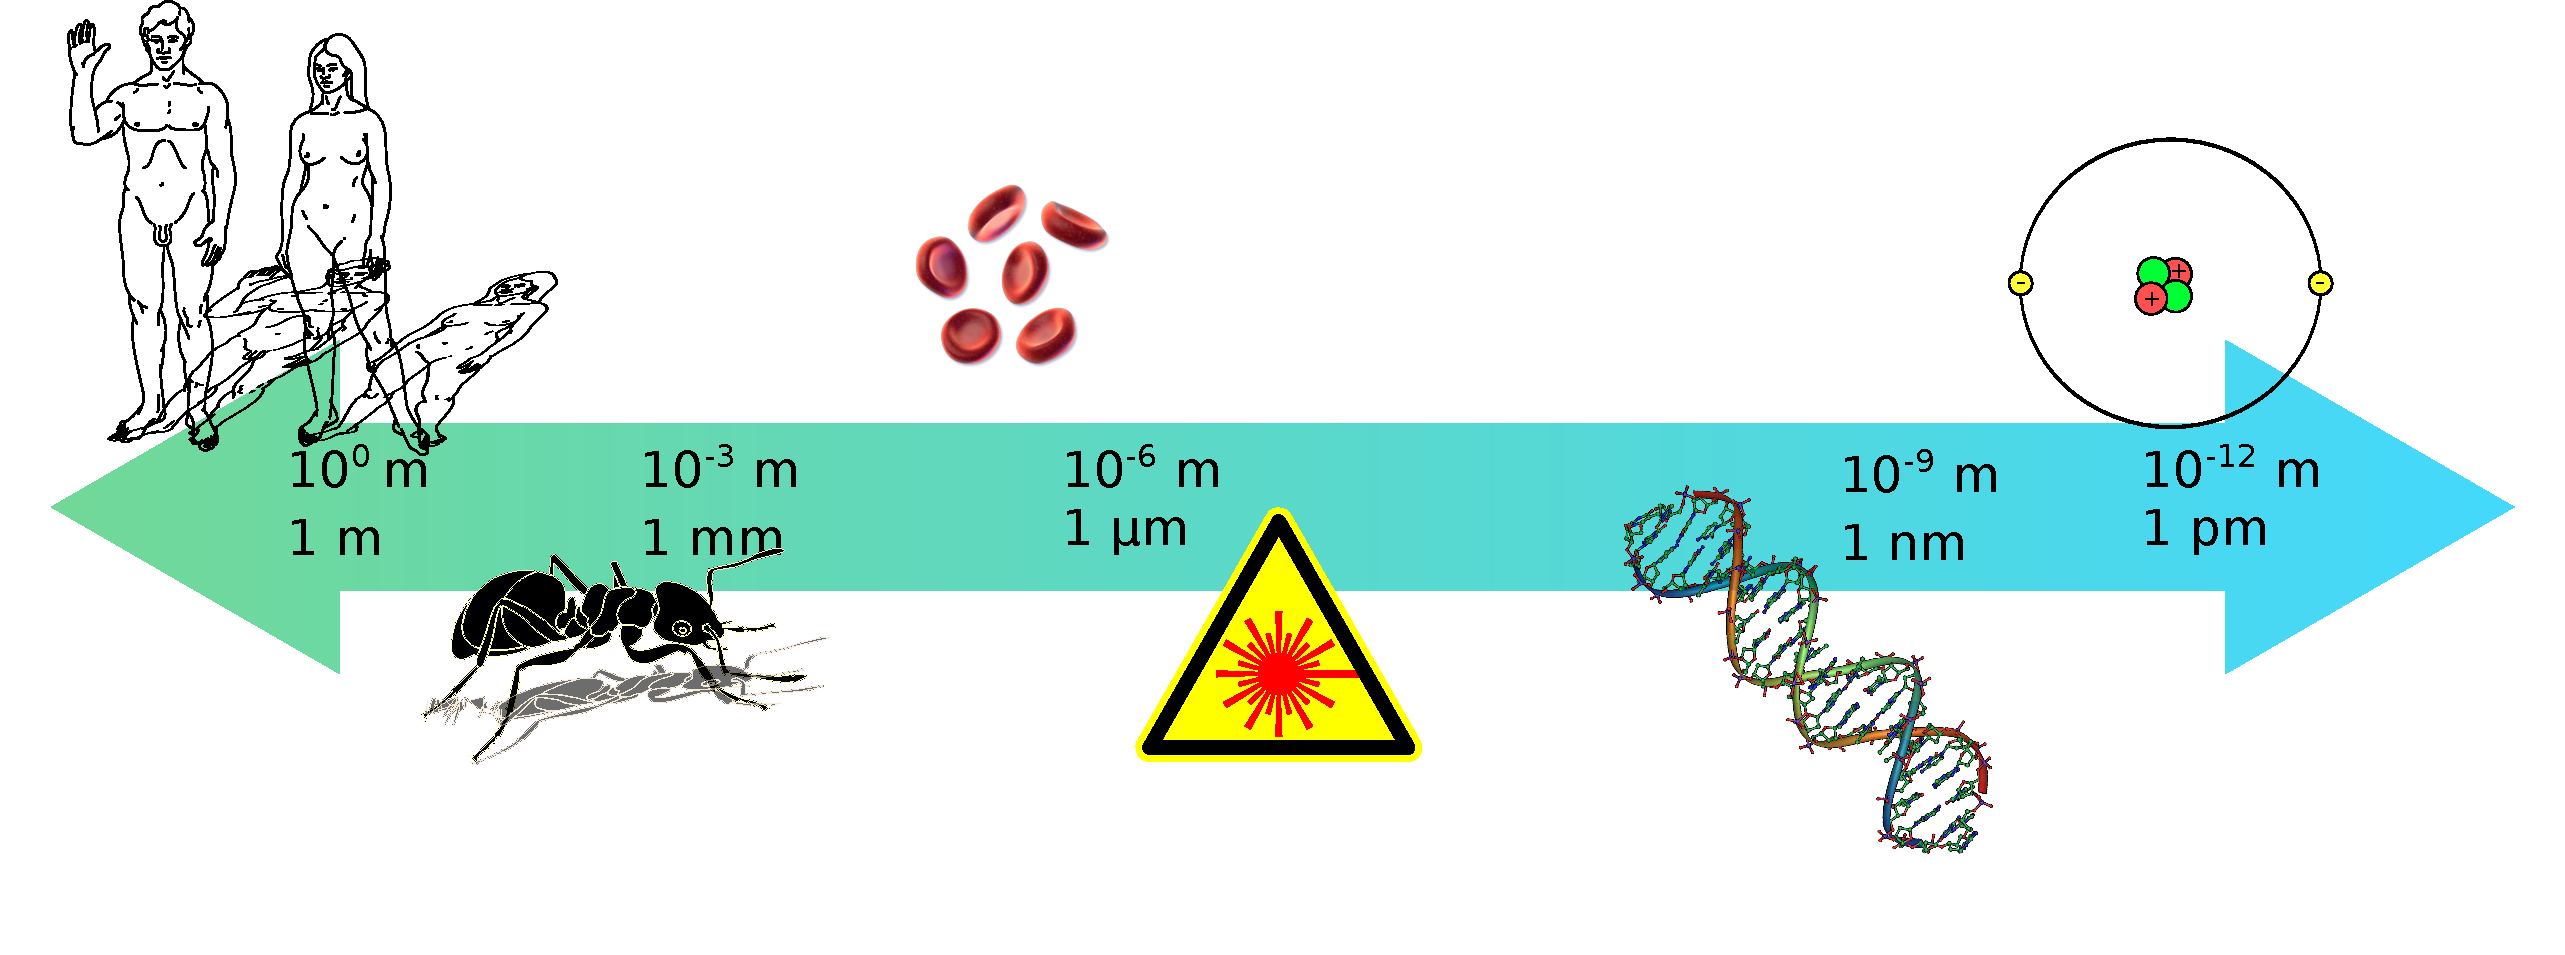
\includegraphics[width=0.9\textwidth]{scale.pdf}
			}
			\caption[Comparativa de ódenes de magnitud desde metros hasta picometros]{Comparativa de órdenes de magnitud. De izquierda a derecha: Escala humana, 1-2 m. Insectos, 10 cm - 1 mm. Glóbulos rojos, 6 $\mathrm{\mu}$m. Longitud de onda de luz visible, 780-380 nm. Transistores en un microprocesador, 100 - 10 nm. Doble hélice de ADN, 2 nm. Radio atómico de un átomo de helio, 31 pm.}
			\label{fig:scale}
		\end{figure}
	\end{frame}

	\begin{frame}{Introducción}
		\begin{figure}
			\centering
			\begin{subfigure}[b]{0.2\textwidth}
				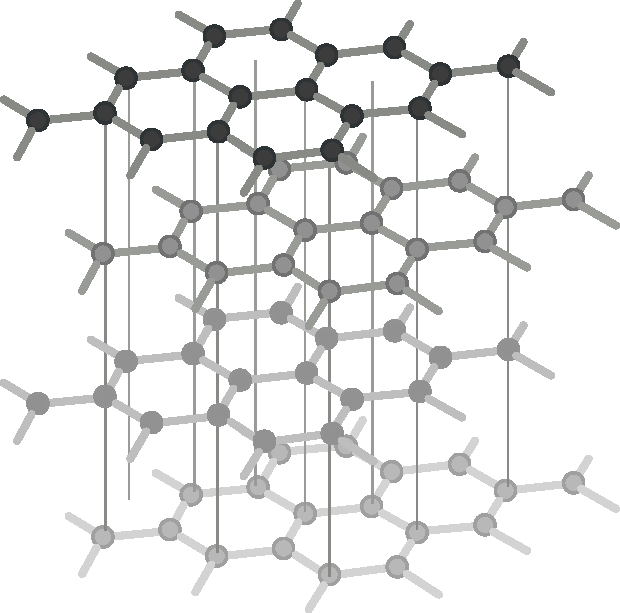
\includegraphics[width=\textwidth]{graphite_structure.pdf}
				\caption{}
				\label{fig:graphite_struct}
			\end{subfigure}
			\begin{subfigure}[b]{0.2\textwidth}
				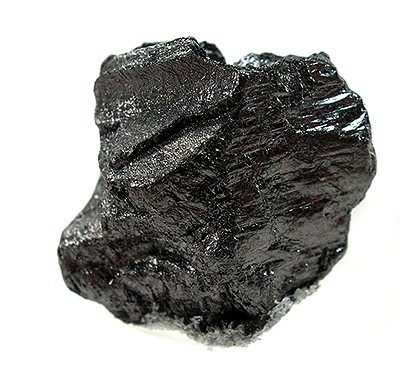
\includegraphics[width=\textwidth]{graphite_image.jpg}
				\caption{}
				\label{fig:graphite_image}
			\end{subfigure}
			\begin{subfigure}[b]{0.2\textwidth}
				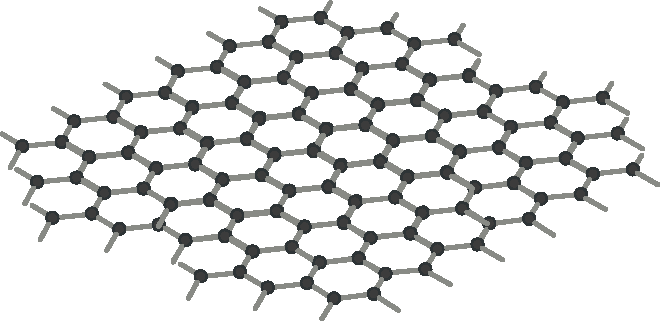
\includegraphics[width=\textwidth]{graphene_structure.pdf}
				\caption{}
				\label{fig:graphene_struct}
			\end{subfigure}
			\begin{subfigure}[b]{0.2\textwidth}
				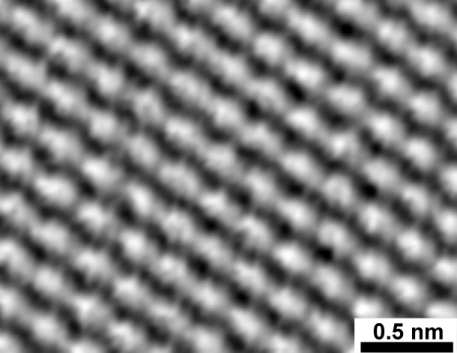
\includegraphics[width=\textwidth]{graphene_image.jpg}
				\caption{}
				\label{fig:graphene_image}
			\end{subfigure}
			\\
			\begin{subfigure}[b]{0.2\textwidth}
				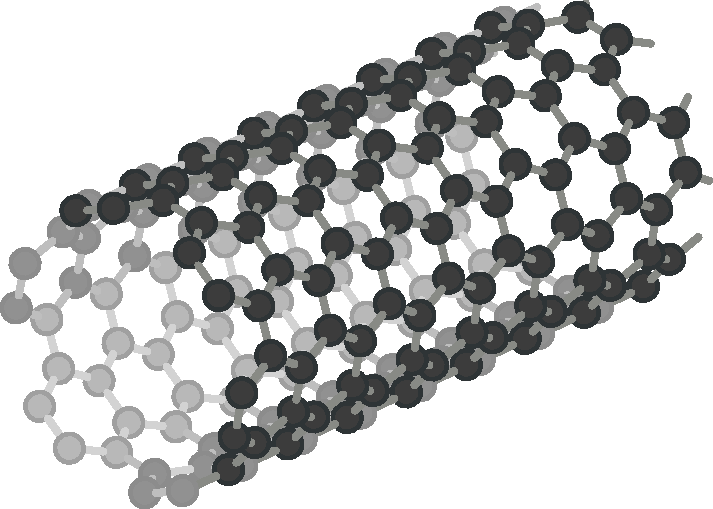
\includegraphics[width=\textwidth]{cnt_structure.pdf}
				\caption{}
				\label{fig:cnt_struct}
			\end{subfigure}
			\begin{subfigure}[b]{0.2\textwidth}
				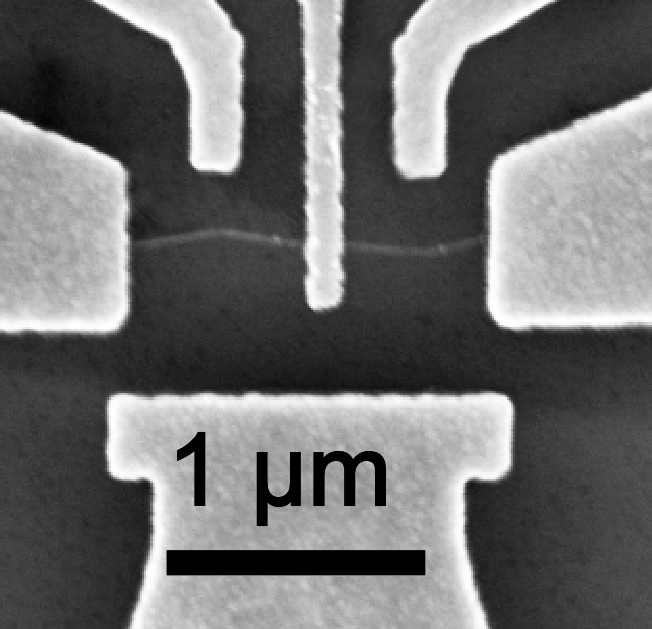
\includegraphics[width=\textwidth]{cnt_image.png}
				\caption{}
				\label{fig:cnt_image}
			\end{subfigure}
			\begin{subfigure}[b]{0.2\textwidth}
				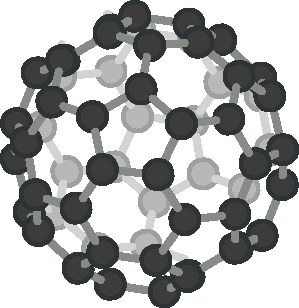
\includegraphics[width=\textwidth]{fullerene_structure.pdf}
				\caption{}
				\label{fig:fullerene_structure}
			\end{subfigure}
			\begin{subfigure}[b]{0.2\textwidth}
				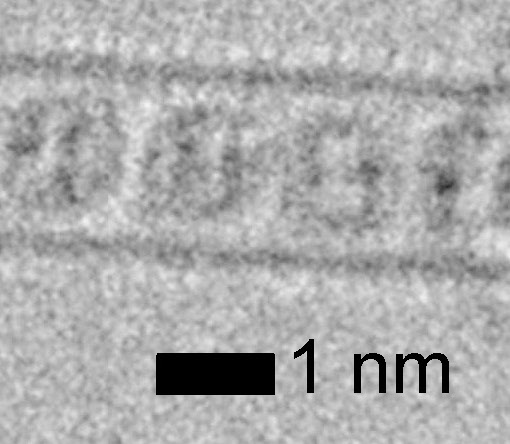
\includegraphics[width=\textwidth]{fullerene_image.jpg}
				\caption{}
				\label{fig:fullerene_image}
			\end{subfigure}
			\caption[Alótropos del carbono mostrando las diferentes dimensionalidades de los nanomateriales]{Estructuras e imágenes de varios alótropos del carbono como ejemplos de la dimensionalidad de los nanomateriales:  \subref{fig:graphite_struct} y \subref{fig:graphite_image} grafito natural, un material 3D. \subref{fig:graphene_struct} y \subref{fig:graphene_image} grafeno, imagen de microscopia de efecto túnel (Frank Trixler, LMU/CeNS: Organic Semiconductor Group), un material 2D. \subref{fig:cnt_struct} y \subref{fig:cnt_image} nanotubo de carbono, imagen SEM de un dispositivo para medir diferentes propiedades del nanotubo (Pavlos Apostolidis, London Centre for Nanotechnology, Department of Physics \& Astronomy), un material 1D. \subref{fig:fullerene_structure} y \subref{fig:fullerene_image} fullereno, imagen TEM de fullerenos C80 funcionalizados dentro de un nanotubo de carbono \citep{Gimenez2011}, un material 0D.}
			\label{fig:carbon_allotropes}
		\end{figure}
	\end{frame}

	\subsection{Grafeno}
	\begin{frame}{Grafeno}
		\begin{figure}
			\centering
			\fbox{
				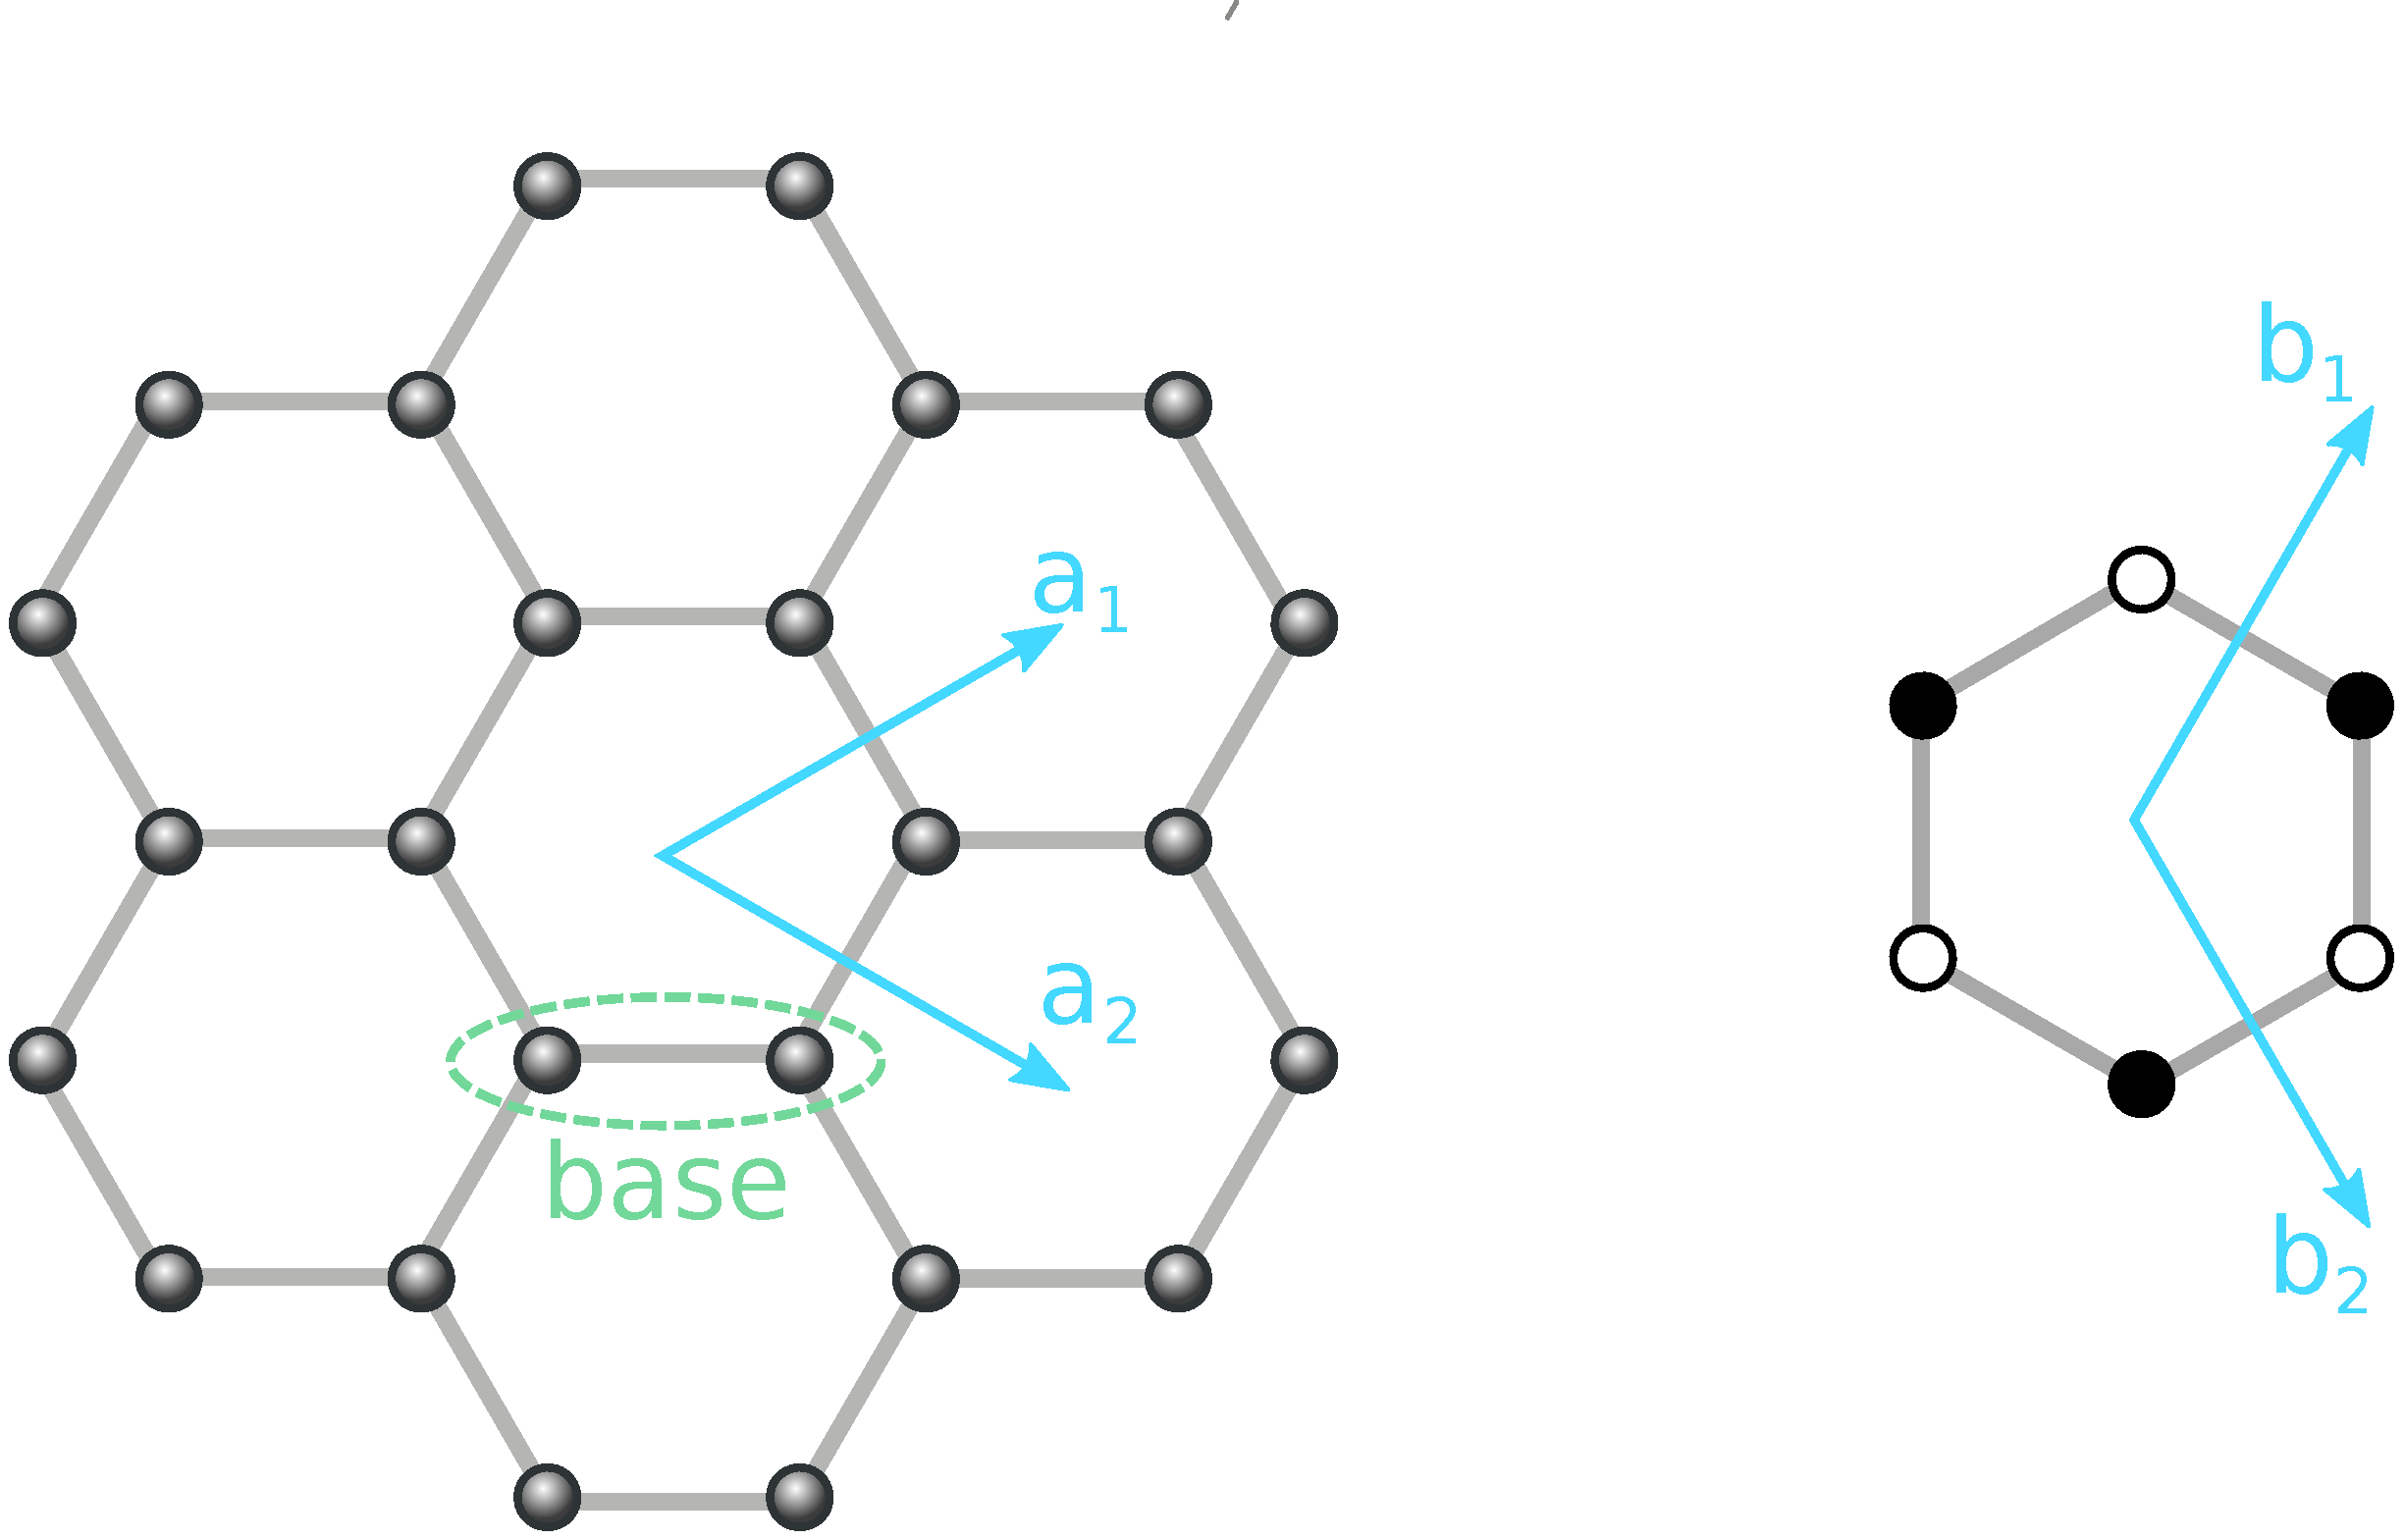
\includegraphics[width=0.75\textwidth]{graphene_lattice.pdf}
			}
			\caption[Estructura cristalina del grafeno]{Izquierda: Red de grafeno en espacio real. Derecha: Red en espacio recíproco.}
			\label{fig_graphene_lattice}
		\end{figure}
	\end{frame}
	
	\subsection{Supercondensadores}
	\begin{frame}{Supercondensadores}
		\begin{figure}
			\centering
			\fbox{
				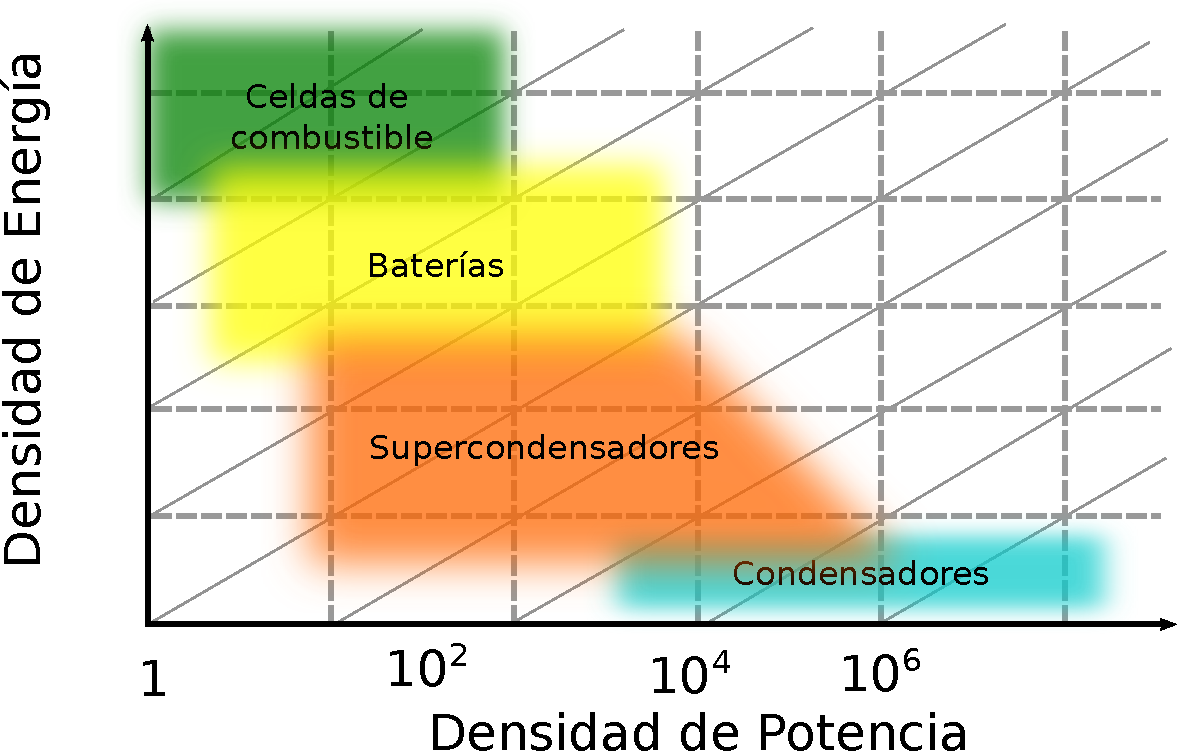
\includegraphics[width = 0.7\textwidth]{ragone.pdf}
			}
			\caption[Diagrama de Ragone, diferentes tecnologías de almacenamiento de energía]{El diagrama de Ragone compara diferentes tecnologías de almacenamiento de energía de acuerdo a su densidad de potencia y densidad de energía.}
			\label{fig:ragone}
		\end{figure}
	\end{frame}

	\section{Ruta de síntesis}
	\begin{frame}{Ruta de síntesis}
%		\begin{figure}
%			\centering
%			\fbox{
%				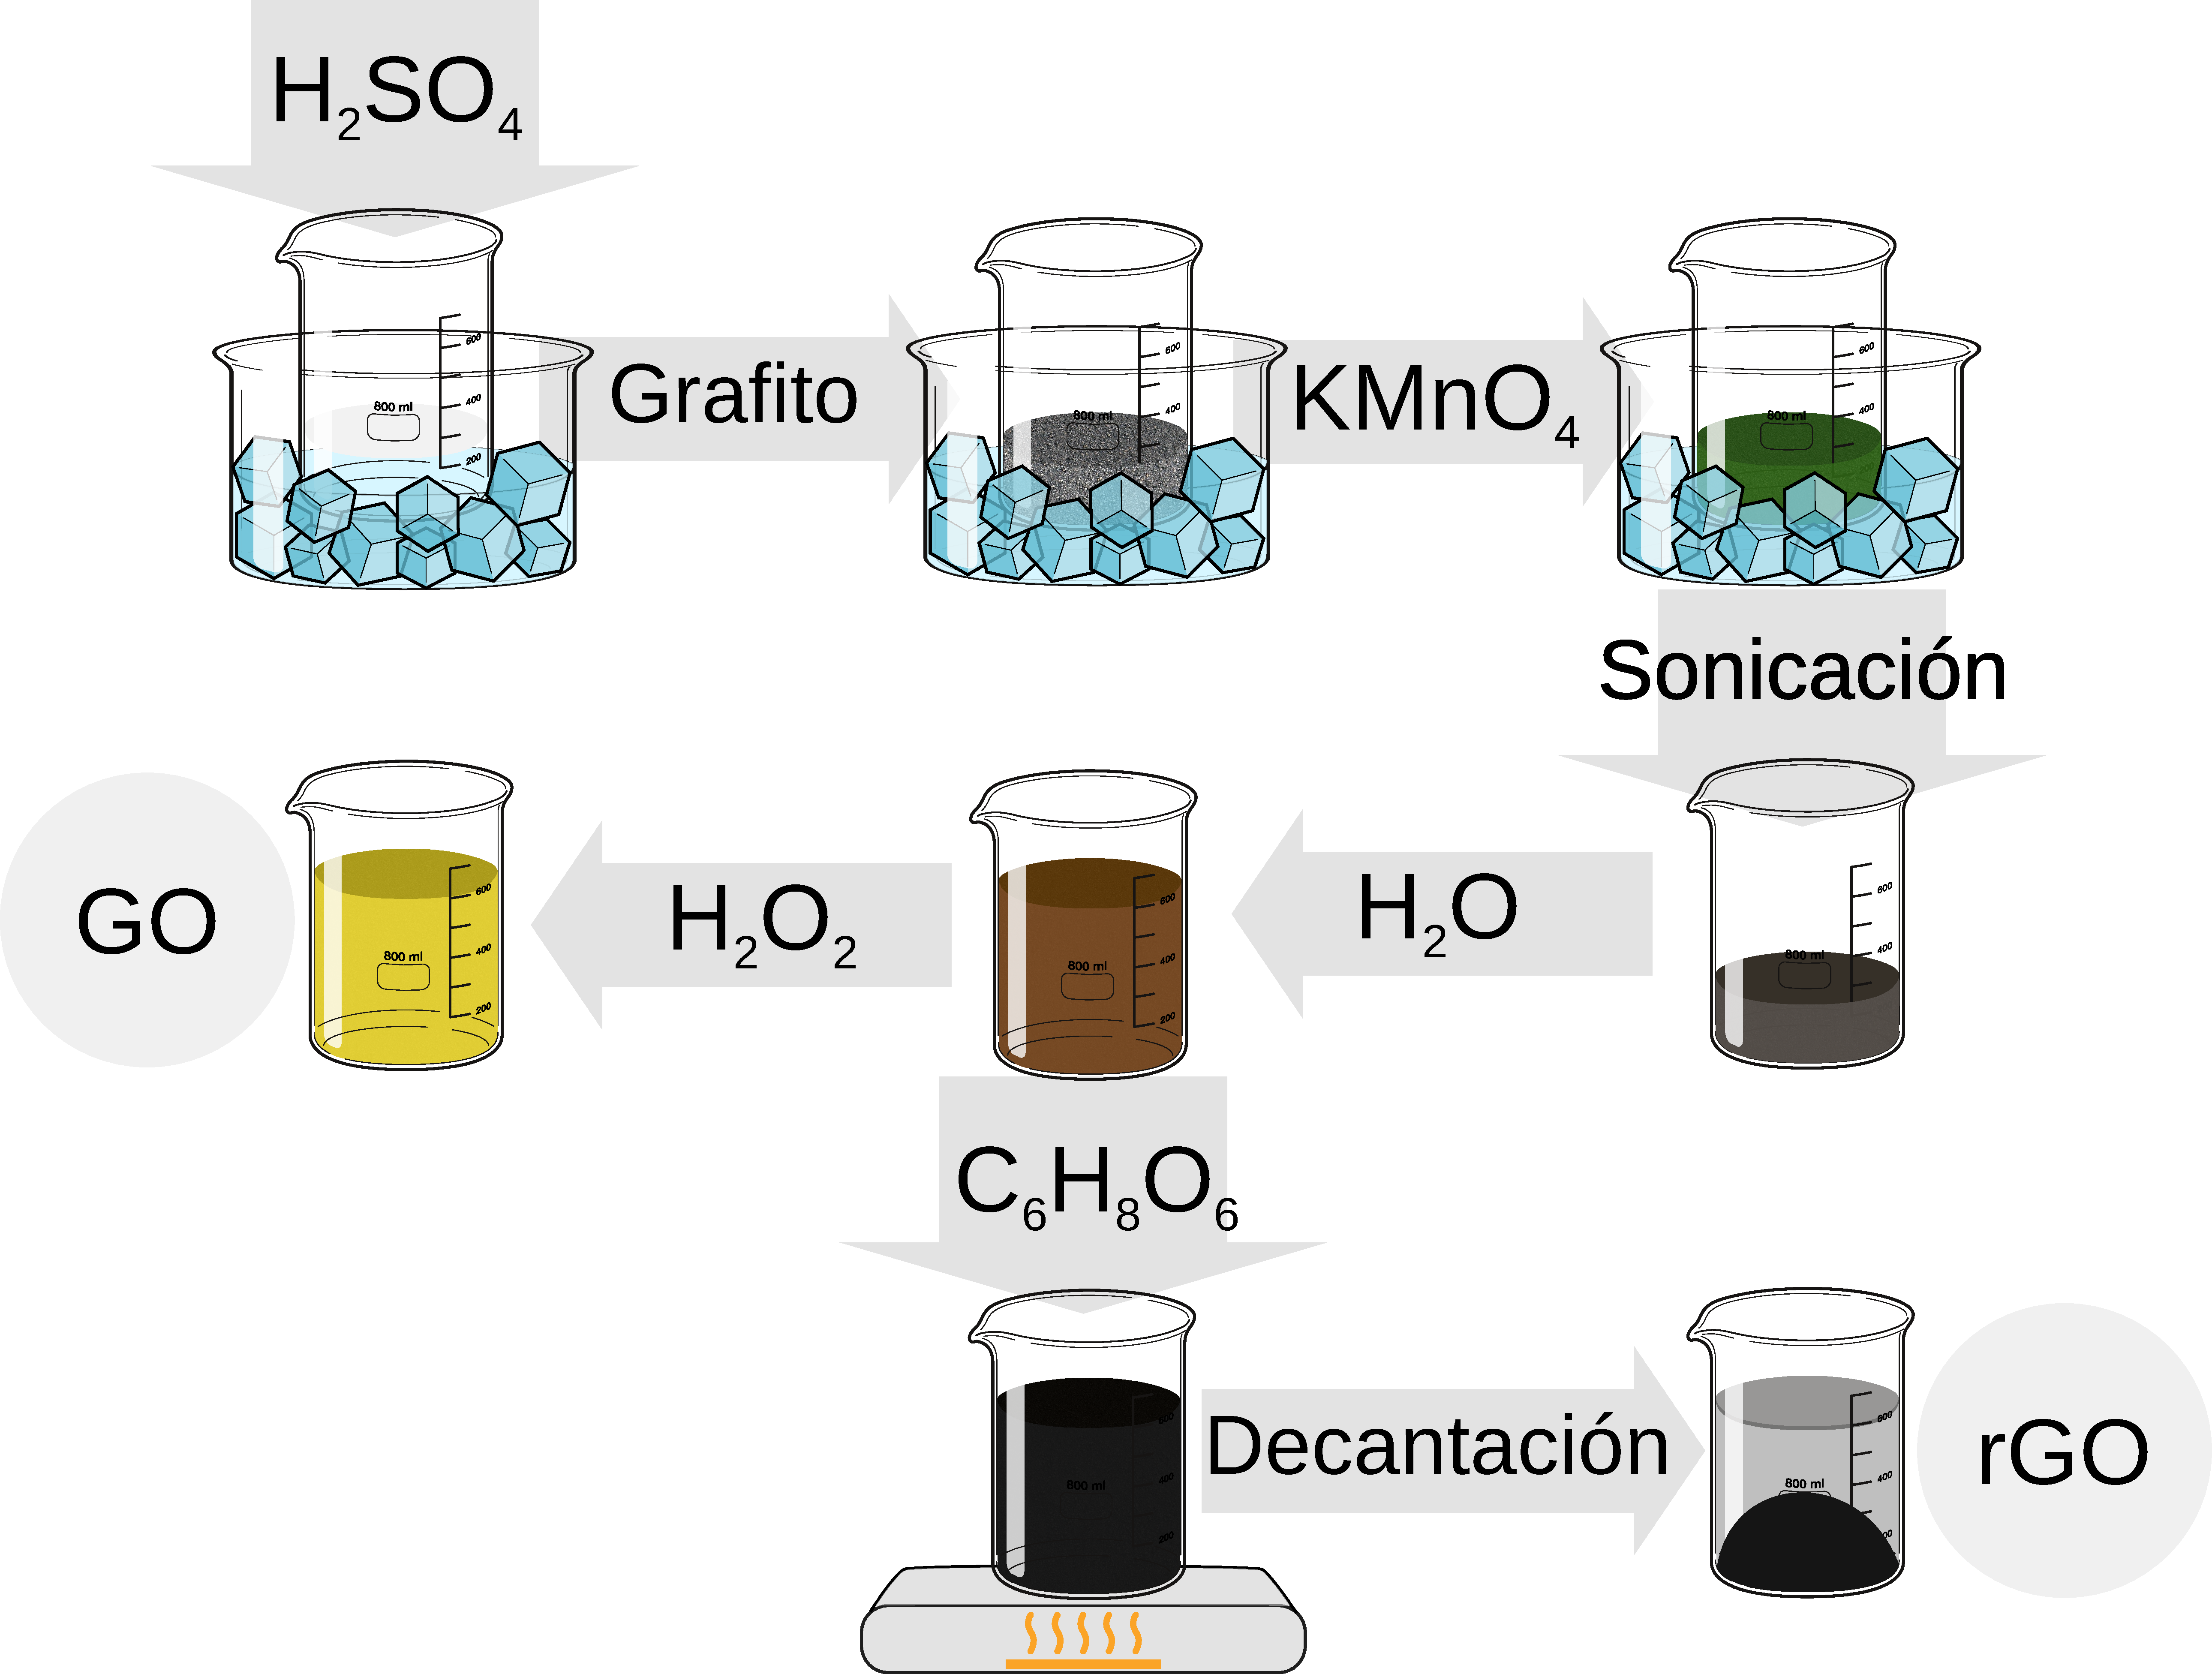
\includegraphics[width=0.8\textwidth]{experimental_method.pdf}
%			}
%			\caption[Método experimental simplicado para la síntesis de óxido de grafeno y óxido reduxido de grafeno]{Método experimental simplificado para la síntesis de óxido de grafeno y óxido reducido de grafeno.}
%		\end{figure}
		\begin{tikzpicture}[]
		\clip(0,0)circle[x radius=1cm, y radius=1cm];
		\clip(0,0)circle[x radius=2cm, y radius=2cm];
		\node{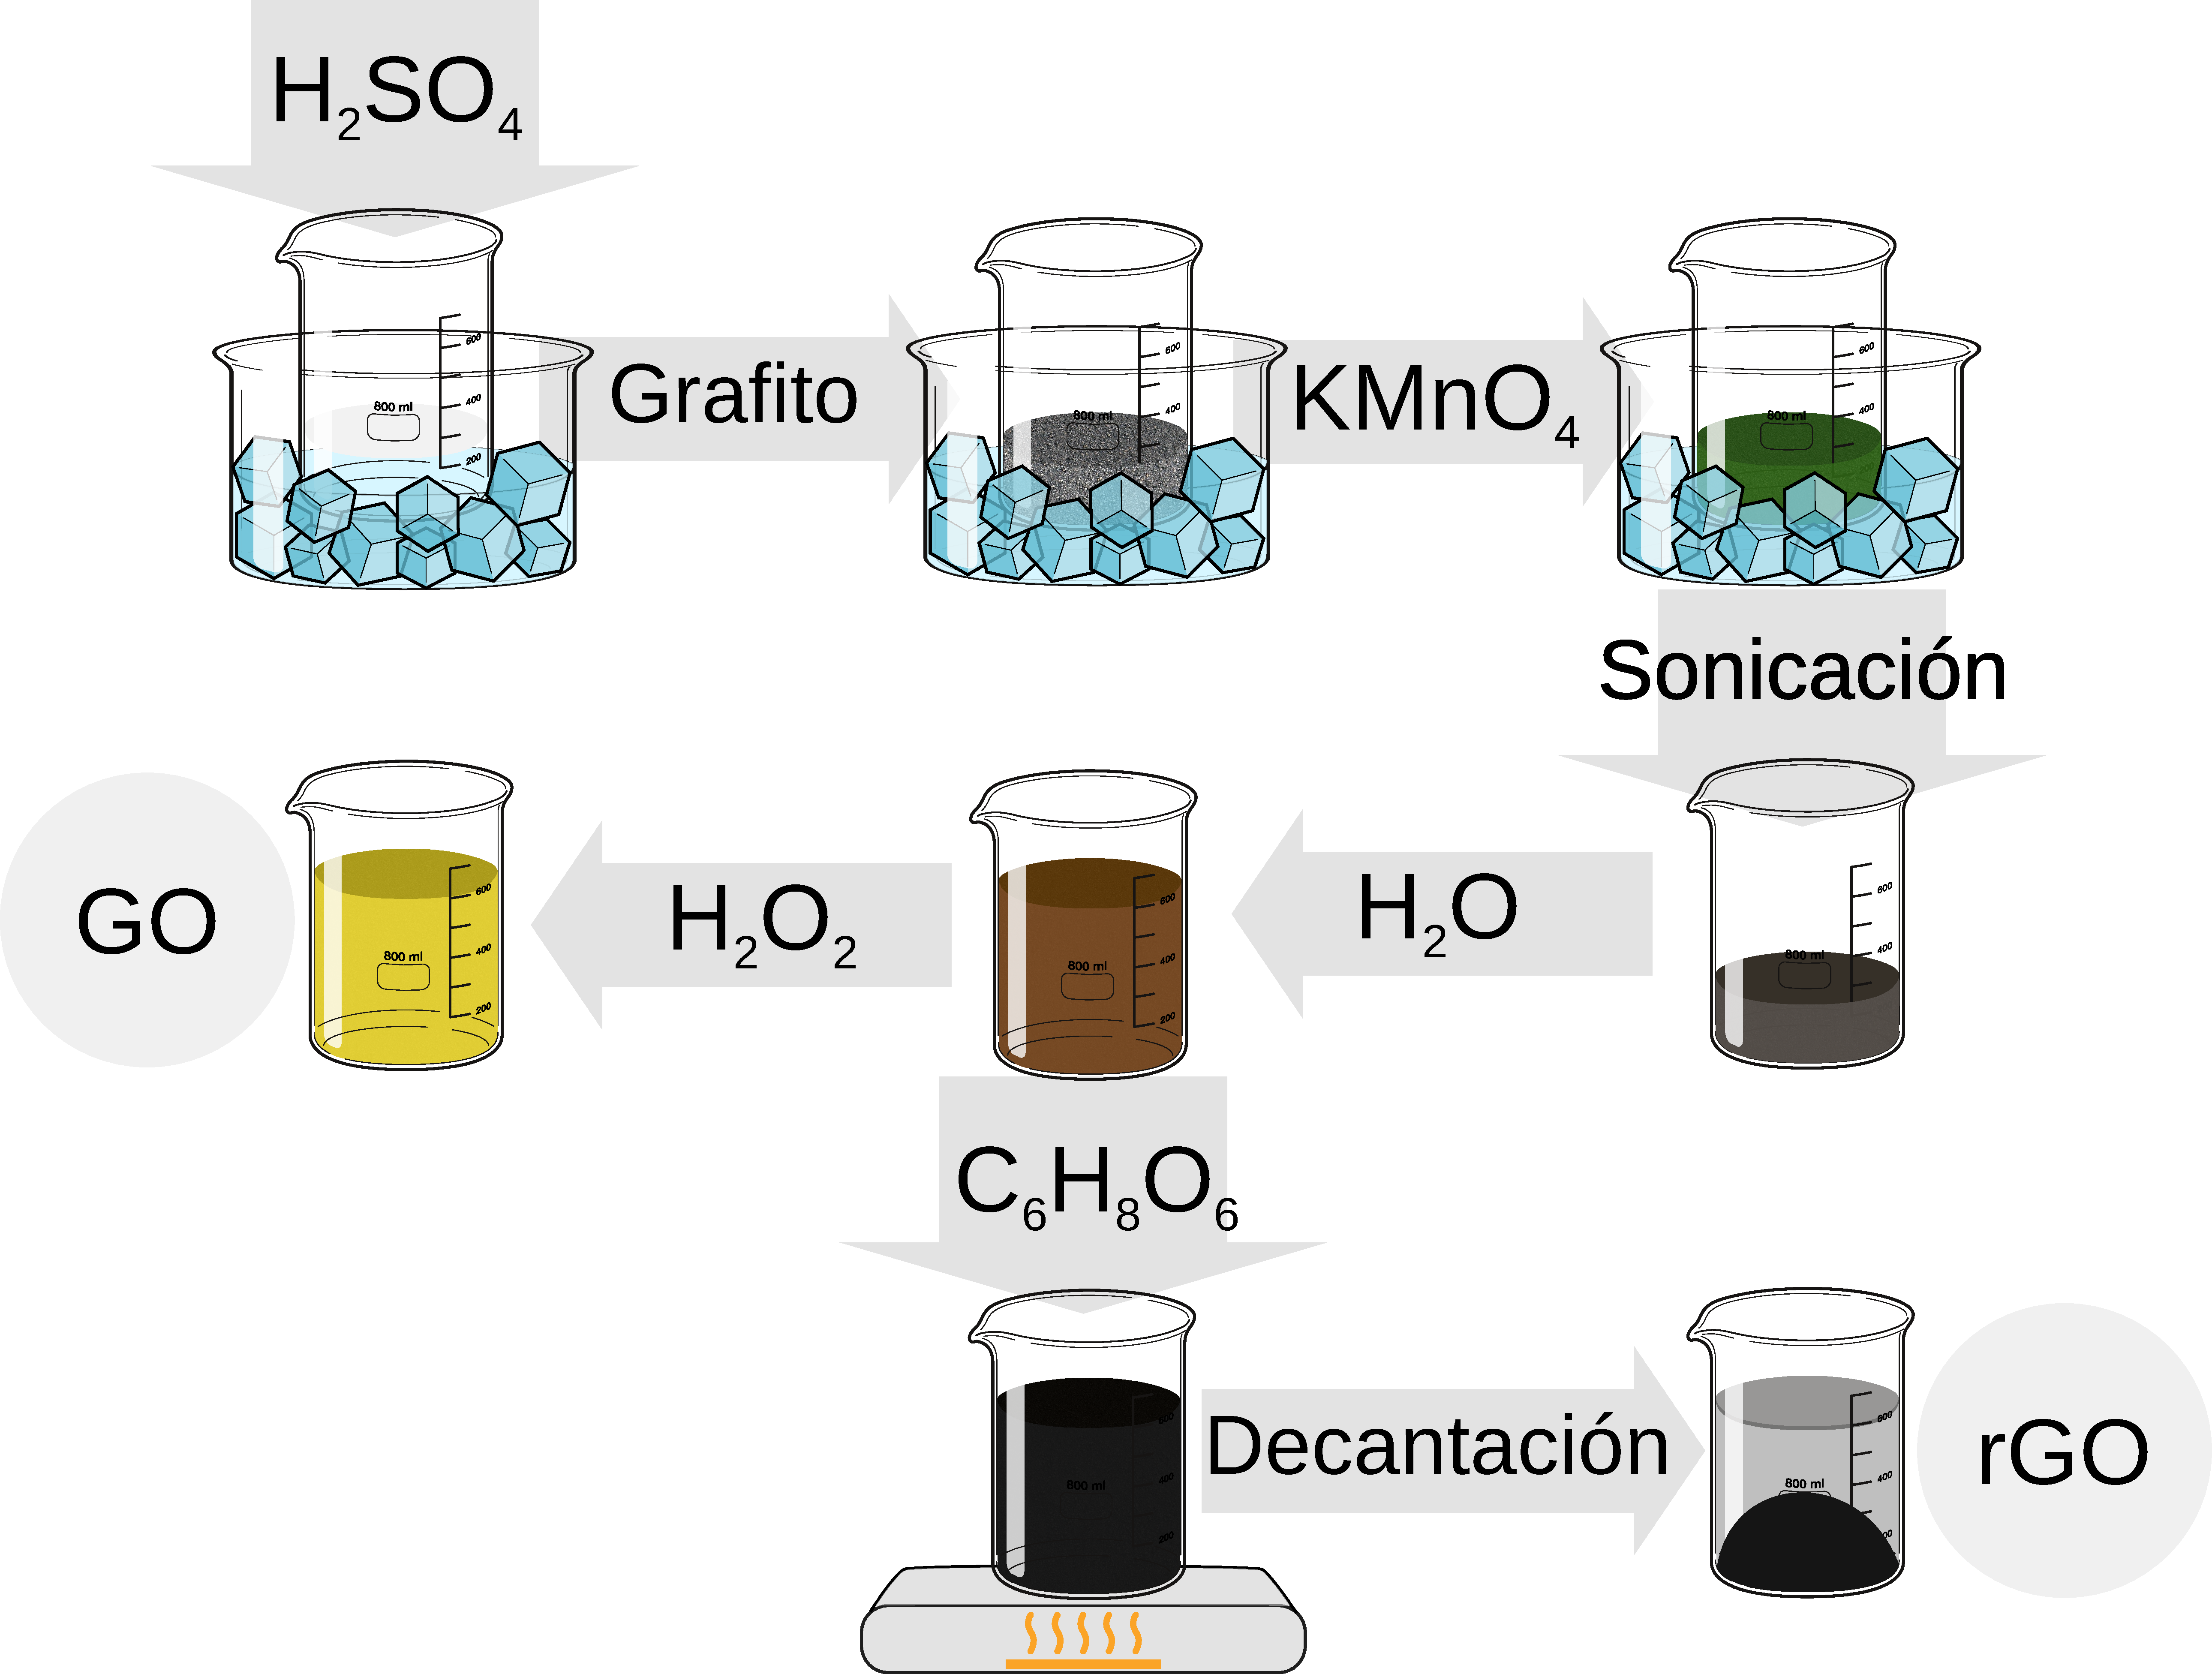
\includegraphics[width=\textwidth]{experimental_method.pdf}};
		\end{tikzpicture}
	\end{frame}
	
	\begin{frame}{XRD}
		\begin{figure}[h]
			\centering
			\begin{tikzpicture}[]
			\begin{axis}[
			cycle list name=colorbrewer-RYB,
			no markers,
			width = 0.8\textwidth,
			yticklabels={,,},
			ylabel={Intensidad},
			y unit=u.a.,
			xlabel={2$\mathrm{\theta}$},
			x unit=grados,
			legend entries={Grafito, Óxido de grafeno, Óxido de grafeno reducido},
			legend style={font=\fontsize{4}{5}\selectfont},
			]
			\addplot table [x expr = \thisrow{2t}, y expr=\thisrow{C}] {./Data/XRD/xrd.txt};
			\addplot table [x expr = \thisrow{2t}, y expr=\thisrow{GO}+1] {./Data/XRD/xrd.txt};
			\pgfplotsset{cycle list shift=1}
			\addplot table [x expr = \thisrow{2t}, y expr=\thisrow{RGO}+2] {./Data/XRD/xrd.txt};
			%	\addplot table [x expr = \thisrow{2t}, y expr=\thisrow{RGOLYO}+3] {./Data/XRD/xrd.txt};
			\node[black, rotate=90] at (24, 0.3){\Tiny{(002)}};
			%	\node[black, rotate=90] at (7, 1.5){\small{10,2\degree}};
			%	\node[black, rotate=90] at (26, 3){\small{22,6\degree}};
			\end{axis}
			\end{tikzpicture}
			\caption[Espectro de difracción de rayos x de grafito, GO y rGO]{Espectro de difracción de rayos x.}
			\label{fig:xrd}
		\end{figure}
	\end{frame}


	

	\section{Bibliografía}
	\begin{frame}{Bibliografía}
		\bibliography{Nanosintesis}
		\bibliographystyle{apalike}
		
	\end{frame}

\end{document}